\section{Supervised learning}
Supervised learning is a subfield of machine learning that refers to training a model to predict a specific target value based on input data.
In this context, the input data is commonly referred to as "features", and when paired with the corresponding target value for prediction, the training is supervised.
There are two types of supervised learning, regression and classification. 
In regression, we predict a continous variable, while we in claffication predict a binary value, true or false.
The model architecture of the model can be the same regardless of predicting a true/false or continuous value. 
The difference is in the loss function, which is used to evaluate the performance of the model during training, and for neural networks, the last layer activation function.
In depth explanations of this will come in the following sections.

\section{Loss/Cost}
In machine learning, the loss of a model refers to the discrepancy between the predicted and true value.
It is calculated using a specific function designed to penalize incorrect predictions and serves as a measure of the model's performance.
The ultimate goal of any machine learning model is to minimize the loss and thereby reduce the difference between predicted and desired outputs.
To achieve this, the model is trained by calculating the gradient of the loss function with respect to different components in the model.
These gradients are then used to determine how the model can be adjusted in the direction that minimizes the loss, through an iterative process.
As a result, the model is optimized to make better predictions and achieve higher accuracy.\\

The most common loss function for regression is the mean squared error
\begin{equation} \label{eq:mse}
    \mathcal{L}(y, \Tilde{y}) = \frac{1}{N}\sum_{i=1}^N(y-\Tilde{y})^2
\end{equation}














\subsection{Loss Functions}
Loss functions are used to evaluate the performance of the machine learning model during training.

In this specific problem, when trying to predict the offset in both azimuth and elevation, there are two obvious ways to calculate the loss.
One where the machine learning model considers the offset in azimuth and elevation separately, and one where it considers both of them together.
Let $\Tilde{y}_{Az}$ and $\Tilde{y}_{El}$ denote the prediction for the offset in azimuth and elevation respectively.
$y_{Az}$ and $y_{El}$ are the true values.
The first way to calculate is 
\begin{equation}\label{eq:mse1}
    \mathcal{L} = \frac{1}{N}\sum_i^N (y_{Az,i}-\Tilde{y}_{Az,i})^2 + \frac{1}{N}\sum_i^N (y_{El,i}-\Tilde{y}_{El,i})^2
\end{equation}
Using this loss function, the machine learning model will focus on minimizing both of the offsets evenly.\\

For the second loss function, we use the mean squared Cartesian distance
\begin{equation}\label{eq:totaloff}
    \mathcal{L} = \frac{1}{N}\sum_i^N \left[ (y_{Az,i}-\Tilde{y}_{Az,i})^2 + (y_{El,i}-\Tilde{y}_{El,i})^2 \right],
\end{equation}

which should have the effect of minimizing the offsets evenly.

\section{Train/test set}
Machine learning models can be highly complex and can fit all the data points in a dataset.
While this can result in perfect predictions on the training data, it often leads to poor performance on new data, a phenomenon known as overfitting.
To counteract this, the data is typically split into two parts - a training set and a test set (sometimes a third validation set is also used).
The model is trained on the training set, and the error on the test set is used to evaluate the model's performance.
By using a separate set of data for testing, we can get a better estimate of the model's performance on new data and avoid overfitting.

When the error on the training data is low, the model has low bias.
However, if the model is too complex, it may also have high variance, meaning that it is overly sensitive to the training data and unable to generalize well to new data.
A model with high variance may perform well on the training data, but its performance on new data may be poor.
The key to building a good model is to balance bias and variance, and to find the right level of complexity that will allow the model to generalize well.
Proper selection of the train/test split ratio and the use of other techniques such as regularization can help achieve this balance and improve the model's performance.


\section{Scaling}

In machine learning, some models such as neural networks are highly sensitive to the scale of input data.
The inputs to a model often contain different types of data with varying scales.
Neural networks use weights to transform the input data, and each neuron in a fully connected network receives data from every input feature.
If the input features have different scales, training the weights can be slow and unstable.
Scaling the input data to have the same scale improves the speed and performance of the model.
In contrast, tree-based models are not affected by the range scale of the data since they consist of tests and not mathematical operations.

The most common scaling method is to standardize the data to have zero mean and a standard deviation of one.
This is achieved by subtracting the mean and dividing by the standard deviation.
Mathematically, the standardization of a feature $x$ is represented as:

\begin{equation}
x_{scaled} = \frac{x - \mu}{\sigma}
\end{equation}

where $\mu$ is the mean of the feature values, and $\sigma$ is the standard deviation of the feature values.
The mean and standard deviation are computed using the following equations:

\begin{align}
\mu &= \frac{1}{n}\sum_{i=1}^{n}x_i\\
\sigma &= \sqrt{\frac{1}{n}\sum_{i=1}^{n}(x_i - \mu)^2}
\end{align}

where $n$ is the number of observations in the feature.
In addition to standardization, other scaling methods such as min-max scaling and robust scaling are also used in specific cases.
Overall, scaling is a crucial step in preprocessing data for machine learning, as it can significantly impact the performance of a model.



\section{Decision Trees}
Decision trees are tree-like models that make decisions based on conditions.
As shown in Figure \ref{fig:decitiontree}, each circle represents a node with various types, including decision nodes that split into two other nodes and leaf/terminal nodes that don't.
The root node is the topmost decision node.
Given an observation, there is a single path to a leaf node that represents the prediction made by the decision tree.

Trees are constructed greedily from the top, meaning that each split is made to minimize the loss function at the current step, without considering future splits.
Single decision trees are not typically sufficient for complex problems.
There are various methods to improve decision tree models, as demonstrated in Figure \ref{fig:evolution_of_xgb}.
The final step in the figure is XGBoost (Extreme Gradient Boost), a highly efficient and high-performing machine learning algorithm.
In this section, we'll briefly cover the methods used to optimize decision trees for prediction.
\cite{Mehta_2019}


\paragraph{Bagging}
Bagging, also known as Bootstrap Aggregation, is a method for training an ensemble of models that contribute to the final prediction.
Each model is trained using bootstrapped data (resampled from the original dataset with replacement), resulting in diverse decision trees.
The final prediction is the average of all ensemble models.

\paragraph{Random Forest}
A method based on bagging, where each tree in the ensemble is made using only a randomly chosen subset of features.
This often leads to better generalization and reduced overfitting.

\paragraph{Boosting}
An ensemble is created in boosting as well, but the trees are not made independently.
They are trained one-by-one considering the previous trees.
A sample weight is assigned to each sample used to train a tree based on the current ensemble's accuracy.
Samples with large prediction error are assigned larger weights and those with accurate predictions are assigned lower weights.
The final prediction is a weighted sum of all ensemble predictions, with weights based on each individual tree's accuracy.

\paragraph{Gradient Boosting}
Like in regular boosting, an ensemble of trees is created iteratively by considering the errors made by previous trees.
The process starts with a constant model that predicts the mean of all samples.
The gradient of the loss function with respect to each sample is calculated and a tree is made to predict these gradients.
The new prediction is the constant plus a small step in the direction of the predicted gradients.
Repeated iteration with small steps in the gradient direction helps reduce both bias and variance.




\begin{figure}[H]
    \centering
    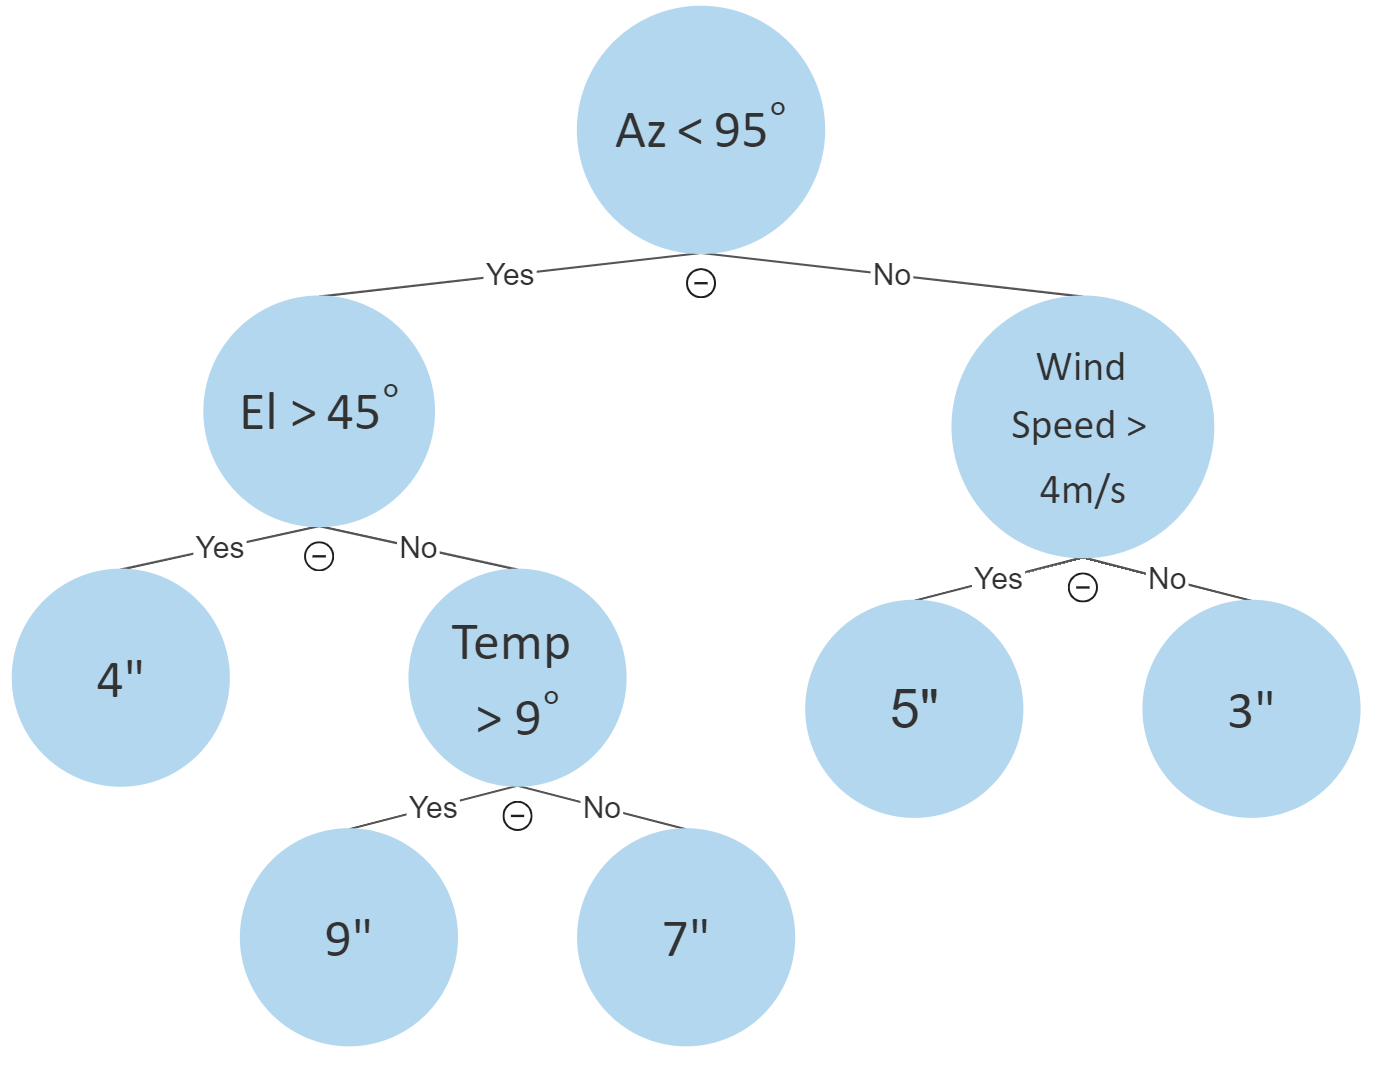
\includegraphics[width=0.98\textwidth]{Other figures/decisiontree_example.PNG}
    \caption{Decision tree with 3 decision nodes and 5 leaf nodes.}
    \label{fig:decitiontree}
\end{figure}

\begin{figure}[H]
    \centering
    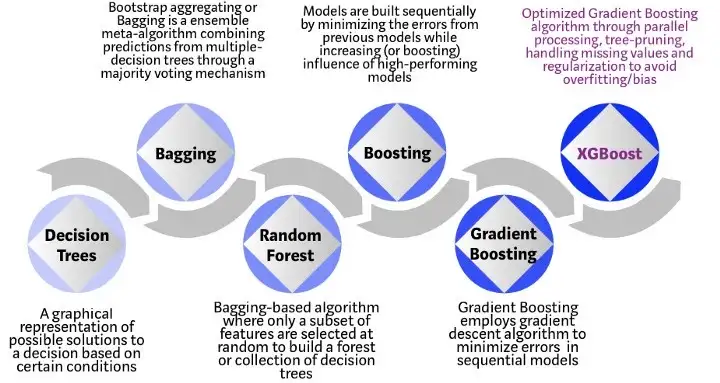
\includegraphics[width=0.98\textwidth]{Other figures/evolution_of_xgb.png}
    \caption{Evolution of XGBoost.
\cite{morde_vishal_nodate}}
    \label{fig:evolution_of_xgb}
\end{figure}

\section{Neural Networks}
A Neural Network (NN) is an Artificial Intelligence (AI) model composed of interconnected neurons, inspired by biological neural networks found in animal brains.
NNs are arranged in layers, as shown in Figure \ref{fig:nnfig}, and consist of an input layer, one or more hidden layers, and an output layer.
The size of the hidden layer(s) varies depending on the nature of the problem.
NNs process input to produce an output, which ideally is close to what you aim to predict.

Each connection in an NN has a trainable weight $w_{jk}^l$, representing the weight from the $k^{th}$ neuron in layer $(l-1)$ to the $j^{th}$ neuron in layer $l$.
Each neuron also has its own bias $b_j$, added to its output to prevent the input to its activation function $\sigma$ from being zero.
The activation function $\sigma$, applied to the neuron's output, is the final transformation before passing data to the next layer.
This nonlinear function is crucial in allowing NNs to learn nonlinear relationships in data \cite{universal_approximation}.

The following is the mathematical explanation of how a neuron processes the outputs from the previous layer.

\begin{equation} \label{eq:act_neuron}
    a_{j}^l = \sigma\left(\sum_k w_{jk}^l a^{l-1}_k+b_j^l \right) = \sigma(z_j^l)
\end{equation}
The quantity 
\begin{equation}\label{eq:z_neuron}
    z_j^l = \sum_{k} w_{jk}^l a^{l-1}_k+b_j^l
\end{equation}
 will be useful explaining how to optimize a neural network, and can be considered the weighted input for neuron $j$ in layer $l$.


\begin{figure}[H]
    \centering
    % NEURAL NETWORK activation
% https://www.youtube.com/watch?v=aircAruvnKk&list=PLZHQObOWTQDNU6R1_67000Dx_ZCJB-3pi&index=1
\begin{tikzpicture}[x=2.7cm,y=1.6cm]
  \message{^^JNeural network activation}
  \def\NI{5} % number of nodes in input layers
  \def\NO{4} % number of nodes in output layers
  \def\yshift{0.4} % shift last node for dots
  
  % INPUT LAYER
  \foreach \i [evaluate={\c=int(\i==\NI); \y=\NI/2-\i-\c*\yshift; \index=(\i<\NI?int(\i):"n");}]
              in {1,...,\NI}{ % loop over nodes
    \node[node in,outer sep=0.6] (NI-\i) at (0,\y) {$a_{\index}^{(0)}$};
  }
  
 

  % OUTPUT LAYER
  \foreach \i [evaluate={\c=int(\i==\NO); \y=\NO/2-\i-\c*\yshift; \index=(\i<\NO?int(\i):"m");}]
    in {\NO,...,1}{ % loop over nodes
    \ifnum\i=1 % high-lighted node
      \node[node hidden]
        (NO-\i) at (1,\y) {$a_{\index}^{(1)}$};
      \foreach \j [evaluate={\index=(\j<\NI?int(\j):"n");}] in {1,...,\NI}{ % loop over nodes in previous layer
        \draw[connect,white,line width=1.2] (NI-\j) -- (NO-\i);
        \draw[connect] (NI-\j) -- (NO-\i)
          node[pos=0.50] {\contour{white}{$w_{1,\index}$}};
      }
    \else % other light-colored nodes
      \node[node,blue!20!black!80,draw=myblue!20,fill=myblue!5]
        (NO-\i) at (1,\y) {$a_{\index}^{(1)}$};
      \foreach \j in {1,...,\NI}{ % loop over nodes in previous layer
        %\draw[connect,white,line width=1.2] (NI-\j) -- (NO-\i);
        \draw[connect,myblue!20] (NI-\j) -- (NO-\i);
      }
    \fi
  }

  %\node[node] (b1) at (0.8, 1.5) {$b_1$};
  \node[bias] (B) at (0.6,1.8) {$b_j^{(1)}$}; 
  \draw[connect,white,line width=1.2] (B) -- (NO-1);
  \draw[connect] (B) -- (NO-1) node[pos=0.50] {\contour{white}{$b_1$}};

  % INPUT LAYER
  \foreach \i in {2,...,\NO}{ % loop over nodes
    \draw[connect, myblue!20, on layer=back] (B) -- (NO-\i);
    }


  % DOTS
  \path (NI-\NI) --++ (0,1+\yshift) node[midway,scale=1.2] {$\vdots$};
  \path (NO-\NO) --++ (0,1+\yshift) node[midway,scale=1.2] {$\vdots$};
  
  % EQUATIONS
  \def\agr#1{{\color{mydarkgreen}a_{#1}^{(0)}}}
  \node[below=17,right=11,mydarkblue,scale=0.95] at (NO-1)
    {$\begin{aligned} %\underset{\text{bias}}{b_1}
       &= \color{mydarkred}\sigma\left( \color{black}
            w_{1,1}\agr{1} + w_{1,2}\agr{2} + \ldots + w_{1,n}\agr{n} + b_1^{(1)}
          \color{mydarkred}\right)\\
       &= \color{mydarkred}\sigma\left( \color{black}
            \sum_{i=1}^{n} w_{1,i}\agr{i} + b_1^{(1)}
           \color{mydarkred}\right)
     \end{aligned}$};
  \node[right,scale=0.9] at (1.3,-1.3)
    {$\begin{aligned}
      {\color{mydarkblue}
      \begin{pmatrix}
        a_{1}^{(1)} \\[0.3em]
        a_{2}^{(1)} \\
        \vdots \\
        a_{m}^{(1)}
      \end{pmatrix}}
      &=
      \color{mydarkred}\sigma\left[ \color{black}
      \begin{pmatrix}
        w_{1,0} & w_{1,1} & \ldots & w_{1,n} \\
        w_{2,0} & w_{2,1} & \ldots & w_{2,n} \\
        \vdots  & \vdots  & \ddots & \vdots  \\
        w_{m,0} & w_{m,1} & \ldots & w_{m,n}
      \end{pmatrix}
      {\color{mydarkgreen}
      \begin{pmatrix}
        a_{1}^{(0)} \\[0.3em]
        a_{2}^{(0)} \\
        \vdots \\
        a_{n}^{(0)}
      \end{pmatrix}}
      +
      \begin{pmatrix}
        b_{1}^{(1)} \\[0.3em]
        b_{2}^{(1)} \\
        \vdots \\
        b_{m}^{(1)}
      \end{pmatrix}
      \color{mydarkred}\right]\\[0.5em]
      {\color{mydarkblue}a^{(1)}}
      &= \color{mydarkred}\sigma\left( \color{black}
           \mathbf{W}^{(1)} {\color{mydarkgreen}a^{(0)}}+\mathbf{b}^{(1)}
         \color{mydarkred}\right)
         %\color{black},\quad \mathbf{W}^{(0)} \in \mathbb{R}^{m\times n}
    \end{aligned}$};
  
\end{tikzpicture}
    \caption{This is an illustration of how information is passed through and processed in a neural network.
Generated using TikZ \cite{tikz}}
    \label{fig:nnfig}
\end{figure}
\subsection{Backpropagation}

Backpropagation\cite{backprop_original} is a fundamental algorithm in training artificial neural networks.
It calculates the gradient of the loss function with respect to all the weights and biases in the network,
allowing for the updating of these parameters in a way that reduces the loss.
The algorithm is based on four key equations, which will be described in this section.\\

We define the error in the $j^\text{th}$ neuron in the $l^\text{th}$ layer by
\begin{equation}\label{eq:bp1} 
    \delta_j^l = \frac{\partial C}{\partial z_j^l} = \frac{\partial C}{\partial a_j^l} \sigma '(z_j^l)
\end{equation}

This can also be considered the partial derivative of the cost function with respect to the bias in neuron $j$ in layer $l$, as 

\begin{equation}\label{eq:bp2}
    \delta_j^l = \frac{\partial C}{\partial z_j^l} = \frac{\partial C}{\partial b_j^l} \frac{\partial b_j^l }{\partial z_j^l} = \frac{\partial C}{\partial b_j^l},
\end{equation}
where we have used the relation $\partial b_j^l / \partial z_j^l = 1$ from rearranging equation \eqref{eq:z_neuron}.
The next equation relates the error in a neuron with the errors in the neurons in the subsequent layer.
\begin{equation}\label{eq:bp3}
    \delta_j^l = \frac{\partial C}{\partial z_j^l} = \sum_k \frac{\partial C}{\partial z_k^{l+1}} \frac{\partial z_k^{l+1}}{\partial z_j^l} = \sum_k \delta_k^{l+1} \frac{\partial z_k^{l+1}}{\partial z_j^l} = \left( \sum_k \delta_k^{l+1} w_{kj}^{l+1} \right) \sigma '(z_j^l)
\end{equation}
Note that the indices on the weight $w$ are now swapped.
We may think of this equation as error propagating backwards by multiplying the error in layer $l+1$ with the transpose of the weight connecting layer $l$ with $l+1$
The final equation is derived from the partial derivative of the cost function with respect to the weight $w_{jk}^l$
\begin{equation}\label{eq:bp4}
    \frac{\partial C}{\partial w_{jk}^l} = \frac{\partial C}{\partial z_j^l} \frac{\partial z_j^l}{\partial w_{jk}^l} = \delta_j^l a_k^{l-1}
\end{equation}

Equation \eqref{eq:bp1} lets us calculate the error in the last layer, and using equation \eqref{eq:bp3} we can propagate this error backwards through the network, calculating the error for all the neurons.
We then use equations \eqref{eq:bp2} and \eqref{eq:bp4} to calculate the gradient of the cost function with respect to the weights and biases.


\subsection{Activation functions}
Activation functions play a crucial role in the training of a neural network by allowing it to learn non-linear relationships between inputs and outputs.
Different activation functions have varying properties, and some of the most common ones will be discussed in this section.
Properties like non-linearity, differentiability, monotonicity, smoothness, and zero-centering are considered important for activation functions.
Non-linearity enables the model to capture complex relationships, differentiability is necessary for calculating the derivative of the loss function with respect to the trainable weights, monotonicity helps ensure stability in activation outputs, smoothness stabilizes gradients during training, and zero-centering balances the activation distribution within the model.

Activation functions play a crucial role in the training of a neural network by allowing it to learn non-linear relationships between inputs and outputs.
Different activation functions have varying properties, and the are some properties considered important.

\begin{itemize}
    \item Non-linearity enables the model to capture complex relationships
    \item Differentiability is necessary for calculating the derivative of the loss function with respect to the trainable weights
    \item Monotonicity helps ensure stability in activation outputs, smoothness stabilizes gradients during training
    \item Smoothness: A smooth activation function helps with making the gradients and training stable.
    \item Zero-centering balances the activation distribution within the model.
\end{itemize}

\paragraph{Tanh}
Tanh, the hyperbolic tangent function is given by
\begin{equation}\label{eq:tanh}
    Tanh(x) = \frac{e^x+e^{-x}}{e^x-e^{-x}}
\end{equation}

\paragraph{ReLU}
The Rectified Linear Unit (ReLU) activation function pushes all negative values to zero while leaving positive values unchanged.
This introduces non-linearity while solving the vanishing gradients problem by having a gradient of either 0 or 1 for negative and positive values, respectively.
\begin{equation}\label{eq:relu}
    R(x) = \begin{cases} x & \mbox{if } x > 0 \\ \mbox{0,} & \mbox{otherwise} \end{cases}
\end{equation}




\section{Model Explainability}
In the context of machine learning, SHAP \cite{SHAP} and SAGE \cite{SAGE} apply the same idea to determine the contribution of each feature to a prediction.
SHAP provides a local explanation by computing the contribution of each feature to the prediction of a single data point.
On the other hand, SAGE provides a global explanation by computing the contribution of each feature to the overall prediction performance of the model.
These methods allow us to understand the relationship between the features and the prediction, which is particularly useful when the model is too complex to interpret.
Additionally, they provide a way to validate the model's fairness and bias.
By understanding which features are contributing the most to a prediction, one can determine if the model is fair or biased, and if the prediction is trustworthy.\\

Both SHAP and SAGE methods are based on Shapley values \cite{shapley_value_1953}, a concept in game theory introduced by Lloyd Shapley in 1951.
Shapley values determine the contribution of each player to a group's surplus or overall value.
The explanation below of Shapley values, SHAP, and SAGE is inspired by a blog post by Ian Covert \cite{covert_shap_sage}.\\

The Shapley value for a player $i$ in a cooperative game with $d$ players is

\begin{equation}
    \phi_i(w) = \frac{1}{d} \sum_{S \subseteq D \backslash \{ i \} } \binom{d-1}{|S|}^{-1} \left[ w(S\cup \{ i \} ) - w(S) \right]
\end{equation}

where $D$ is the set of all players, $S$ is a coalition of players, $w(S)$ is the value of the coalition $S$, and $|S|$ is the number of players in the coalition.
This formula satisfy four important conditions:
\begin{itemize}
    \item Efficiency: The sum of all Shapley values should be equal to the total value of the group.
    \item Symmetry: If two players $i$ and $j$ have the same impact on all coalitions with $w(S \cup \{i\}) = w(S \cup \{j\})$ for all $S$, they should have the same Shapley value $\phi_i(w) = \phi_j(w)$.
    \item Dummy: A player $i$ that makes no contribution to the group with $w(S \cup \{i\}) = w(S)$, should receive a value of zero, or $\phi_i(w)=0$.
    \item Linearity: The value of a player should be proportional to their contribution to the group.
If player $i$ contributes twice as much to the groups overall worth than player $j$, then player $i$ should have twice the Shapley value.
\end{itemize}

\subsection{SHAP}
Shapley values explain how each feature $(x^1, \dots, x^d)$ in a model $f$ contributes to the deviation from the mean prediction $\mathbb{E}[f(x)]$ of the dataset, for a single prediction.
It a assigns a value $\phi_1, \dots, \phi_d$ to each feature, that quantifies the feature's influence on the prediction $f(x)$.
SHAP (Shapley Additive Explanations) is a way of computing approximate Shapley values for machine learning models.\\

We define a cooperative game $v_{f,x}$ to represent a prediction given the features $x^S$, as
\begin{equation}
    v_{f,x}(S) = \mathbb{E} \left[ f(X) | X^S = x^S \right],
\end{equation}

where $x^S$ are known, and the remaining features are treated as random variable $X^{\Bar{S}}$ (where $\Bar{S} = D \backslash S$).
This is the mean prediction $f(X)$ when the unknown values follow the conditional distribution $X^{\Bar{S}} | X^S = x^S$.\\

Using a subset of features from the prediction while sampling the rest from the dataset, reduces the chance of improbable samples.
Given this convention for making predictions, we can apply the Shapley value to define each feature's contribution to the prediction $f(X)$ using Shapley values $\phi_i(v_{f,x})$.
A Shapley value of $\phi_i(v_{f,x}) > 0$ indicates that feature $i$ contributes to an increase in prediction $f(X)$.
A negative Shapley value $\phi_i(v_{f,x}) < 0$ indicates the opposite, that the feature contributes to a decrease in $f(X)$.
Uninformative features will have small values $\phi_i(v_{f,x}) \approx 0$.

\subsection{SAGE}
SAGE (Shapley Additive Global Importance) explains how every feature contributes to the performance of the model overall, and it relates to SHAP in a simple way.
For a given feature, the global feature importance is the average SHAP value (for that feature) across all samples in the dataset.
This is, however, not how it is calculated in practise.
A paper by Ian Covert et al.
\cite{sage_paper} on global feature importance proposes an algorithm that aims directly at a global feature explanation, unlike the SHAP values, which makes
it faster.
This is the algorithm used for approximating the SAGE values for the features in the thesis.

